% ============================================================
% FinMini: EECS 545 Final Project Report
% ============================================================
\documentclass[11pt,letterpaper]{article}

\usepackage[utf8]{inputenc}
\usepackage[T1]{fontenc}
\usepackage[margin=1in]{geometry}
\usepackage{graphicx}
\usepackage{booktabs}
\usepackage{amsmath}
\usepackage{amssymb}
\usepackage{hyperref}
\usepackage{microtype}
\usepackage{subcaption}
\usepackage{multirow}
\usepackage{array}
\usepackage{xcolor}
\usepackage{parskip}
\usepackage{enumitem}
\setlength{\parskip}{4pt}

\hypersetup{
  colorlinks=true,
  linkcolor=blue!60!black,
  citecolor=blue!60!black,
  urlcolor=blue!60!black
}

% ============================================================
\title{\textbf{FinMini: Two-Stage Fine-Tuning of a Compact LLM\\
for Financial Sentiment Analysis and Text-Driven Stock Movement Prediction}}

\author{
  JiaYi Zhang,\; JiaYuan Jiang,\; Yue Yu,\; YiXiang Fei \\[2pt]
  \small\texttt{jiayizha@umich.edu,\; jiayuanj@umich.edu,\;
                yuyuea@umich.edu,\; feiyx@umich.edu} \\[2pt]
  \small Electrical Engineering and Computer Science, University of Michigan \\
  \small EECS 545: Machine Learning, Winter 2026
}
\date{}

% ============================================================
\begin{document}
\maketitle
\thispagestyle{empty}

% ============================================================
\begin{abstract}
Large language models (LLMs) excel at general-purpose tasks yet
consistently underperform in specialized financial domains, where
domain-specific terminology, implicit sentiment cues, and causal
reasoning differ fundamentally from everyday language.
We present \textbf{FinMini}, a two-stage domain adaptation pipeline
applied to the compact 8B-parameter model
\textit{DeepSeek-R1-Distill-Llama-8B}.
The first stage performs quantized LoRA supervised fine-tuning (QLoRA-SFT)
on 63,395 labeled financial samples drawn from three curated corpora.
The second stage extends training with Chain-of-Thought SFT (CoT-SFT),
replacing bare sentiment labels with structured \texttt{<think>} reasoning
traces generated via the DeepSeek API, aligned with the base model's
native format.
Evaluated on four benchmarks from the Open FinLLM Leaderboard ---
FPB, FiQASA, SM-BigData, and SM-CIKM --- FinMini CoT-SFT achieves
\textbf{98.5\%}, \textbf{97.7\%}, \textbf{57.3\%}, and \textbf{55.5\%}
accuracy respectively, outperforming all evaluated baselines including
Mistral-7B-Instruct and Meta-Llama-3-8B-Instruct.
We further demonstrate an end-to-end application by deploying the
fine-tuned model in a quarterly long-short equity strategy over the
S\&P~500 universe, showing that LLM-derived sentiment scores can serve
as meaningful cross-sectional return signals.
\end{abstract}

% ============================================================
\section{Introduction}
\label{sec:intro}

Financial natural language processing (NLP) has long been recognized as
a challenging specialization of general NLP~\cite{du2024survey}.
Financial texts --- earnings call transcripts, analyst reports, news
headlines, and social media posts --- carry domain-specific vocabulary,
tight regulatory conventions, and implicit causal chains that
general-purpose language models are not pretrained to decode.
For instance, the phrase ``earnings in line with expectations'' may signal
a mildly negative outcome to a financial analyst (the stock had already
priced in an upside surprise), yet a general LLM interprets it as neutral.
Lexicon-based methods such as the Loughran--McDonald
dictionary~\cite{loughran2011liability} addressed the vocabulary mismatch
but cannot capture context-dependent sentiment.

The rapid proliferation of open-source instruction-tuned LLMs raises a
natural question: \emph{can a compact, freely available model be
efficiently adapted to match or exceed the financial NLP performance of
much larger proprietary systems?}
We focus on two closely related tasks.
\textbf{Financial sentiment analysis} asks whether a piece of financial
text carries a positive or negative market-relevant signal.
\textbf{Stock movement prediction} asks whether the referenced asset will
rise or fall given textual evidence.
Both tasks are framed as binary classification under a unified
positive/negative scheme following the Open FinLLM
Leaderboard~\cite{huang2024openfinllms}.

Our main contributions are:
\begin{enumerate}[itemsep=1pt]
  \item A \textbf{two-stage fine-tuning pipeline} combining QLoRA-SFT
        and CoT-SFT for parameter-efficient domain adaptation of a
        compact reasoning-distilled LLM.
  \item A \textbf{CoT data augmentation strategy} that leverages the
        DeepSeek API to synthesize structured \texttt{<think>} reasoning
        traces for over 60,000 financial training samples, aligned with
        the base model's native output format.
  \item Comprehensive \textbf{benchmarking} of three open-source 7--8B
        models in zero-shot mode, with staged ablation across fine-tuning
        phases.
  \item An \textbf{end-to-end trading strategy demonstration} that
        applies the fine-tuned model to S\&P~500 earnings call scoring
        and constructs a quarterly long-short equity portfolio.
\end{enumerate}

% ============================================================
\section{Related Work}
\label{sec:related}

\textbf{Lexicon-based and classical methods.}
Early work on financial sentiment relied on domain-adapted lexicons such
as the Loughran--McDonald dictionary~\cite{loughran2011liability} and
traditional classifiers (SVM, logistic regression) applied to bag-of-words
features~\cite{cam2024twitter}.
These approaches capture vocabulary mismatches between general English and
financial jargon but cannot model context, negation, or causal chains.

\textbf{FinBERT}~\cite{araci2019finbert} established domain-specific
pre-training as the baseline for financial NLP, showing that a BERT model
fine-tuned on financial corpora substantially outperforms general-purpose
models on sentiment classification.
However, BERT-family models operate at the encoder level and lack the
instruction-following and chain-of-thought capabilities of modern
decoder-only LLMs.

\textbf{BloombergGPT}~\cite{wu2023bloomberggpt} trained a 50B-parameter
model from scratch on 700B tokens of financial text, achieving strong
performance across diverse financial tasks.
While impressive, this approach requires massive proprietary data and
infrastructure, motivating parameter-efficient alternatives.

\textbf{PIXIU}~\cite{xie2023pixiu} introduced FinBen, a comprehensive
financial instruction-tuning dataset and benchmark covering sentiment
analysis, information extraction, and question answering.
It demonstrated that supervised fine-tuning on diverse financial tasks
yields competitive results on the Open FinLLM Leaderboard --- the
framework we adopt.
Our training data partially overlaps with PIXIU's FPB source but
extends it with the large-scale FinGPT/Twitter corpus~\cite{wang2023fingpt}
and stock movement data for broader task coverage.

\textbf{Long CoT SFT}~\cite{ou2025cot} showed that chain-of-thought
supervised fine-tuning is a prerequisite for instilling robust reasoning
in lightweight LLMs, outperforming reinforcement learning as a standalone
strategy.
This directly motivates our second fine-tuning stage: rather than RL-based
approaches, we inject reasoning capability through structured supervised
data aligned with the base model's native format.

% ============================================================
\section{Method}
\label{sec:method}

\subsection{Base Model Selection}

We select \textbf{DeepSeek-R1-Distill-Llama-8B} as our base model for
three reasons.
First, it incorporates reasoning-distillation pretraining, which endows
it with stronger structured reasoning out of the box compared with
standard instruction-tuned models.
Second, among zero-shot baselines (Section~\ref{sec:experiments}),
it achieves the highest average accuracy on social-media benchmarks,
suggesting a better-initialized prior for ambiguous financial text.
Third, its native \texttt{<think>}\ldots\texttt{</think>} output format
is directly compatible with our CoT-SFT augmentation strategy.

\subsection{QLoRA Supervised Fine-Tuning}
\label{subsec:qlora}

We apply \textbf{QLoRA}~\cite{dettmers2024qlora} to reduce memory
footprint while preserving model quality.
The base model is loaded in 4-bit NF4 double quantization
(bitsandbytes), keeping all original weights frozen.
Low-rank adapter matrices are injected into all seven projection
matrices: \texttt{q\_proj}, \texttt{k\_proj}, \texttt{v\_proj},
\texttt{o\_proj}, \texttt{gate\_proj}, \texttt{up\_proj},
\texttt{down\_proj}.
Formally, for a pretrained weight matrix $W_0 \in \mathbb{R}^{d\times k}$,
the adapted forward pass is:
\[
  h = W_0 x + \frac{\alpha}{r} B A x,
  \quad A \in \mathbb{R}^{r \times k},\; B \in \mathbb{R}^{d \times r},
\]
where rank $r=16$ and scaling factor $\alpha=32$.
Only $A$ and $B$ are updated during training, reducing trainable
parameters from $\sim$8B to $\sim$42M while maintaining full model
expressiveness via the quantized base.

\textbf{Training configuration.}
We train for 3 epochs with per-device batch size 4 and gradient
accumulation of 4 steps (effective batch size 16), using
paged AdamW at learning rate $2\times10^{-4}$ with a cosine decay
schedule.
Maximum sequence length is 512 tokens with BF16 mixed precision.

\subsection{Training Corpus}

\begin{table}[ht]
\centering
\small
\begin{tabular}{@{}lrp{6.2cm}@{}}
\toprule
\textbf{Dataset} & \textbf{Samples} & \textbf{Selection Rationale} \\
\midrule
FPB (Financial PhraseBank) & 2,264 & 100\% inter-annotator agreement;
  gold-standard annotation quality \\
DS2 (FinGPT + Twitter~\cite{wang2023fingpt}) & 100,037 & Multi-source scale;
  covers news, social media, and analyst commentary \\
FLARE-SM-ACL & 27,056 & Stock movement reasoning;
  extends task diversity beyond pure sentiment \\
\midrule
\textbf{Total (train / test split)} & \textbf{63,395 / 7,979} & \\
\bottomrule
\end{tabular}
\caption{Training corpus. Positive/negative class distribution:
  41,211 / 22,184 in train; 5,235 / 2,744 in test.
  Neutral labels are removed to unify the binary classification framework.}
\label{tab:data}
\end{table}

Each sample follows an instruction/input/output template.
The instruction describes the task; the input contains the financial text;
the output is the sentiment label (\texttt{positive} / \texttt{negative}).
Proportional sampling is applied so that the large DS2 corpus does not
overwhelm the high-quality FPB annotations.

\subsection{Chain-of-Thought Supervised Fine-Tuning}
\label{subsec:cot}

The first-stage adapter is retained and training continues on a
CoT-augmented version of the corpus.
For each training sample, we query \textbf{DeepSeek-chat}
(temperature 0.7, \texttt{max\_tokens}$=300$) to generate a structured
reasoning chain.
The output format is transformed from a bare label into:
\[
  \texttt{<think>}\;\text{[financial reasoning]}\;\texttt{</think>}\;
  \texttt{positive} \mid \texttt{negative}
\]
Training uses \texttt{completion\_only\_loss}: only the completion
tokens --- the \texttt{<think>} trace plus the final label --- contribute
to the gradient, not the prompt.
Maximum sequence length is extended to 2,048 tokens to accommodate
reasoning traces.
After quality filtering and a 90/10 split, 54,595 / 6,067 samples are
used for this stage.

Figure~\ref{fig:loss} shows the training loss curves for both stages.
The first stage converges from ${\sim}4.0$ to ${\sim}1.8$;
the second stage converges from ${\sim}1.0$ to ${\sim}0.5$,
reflecting the richer supervision signal provided by reasoning traces
compared with label-only outputs.

\begin{figure}[ht]
\centering
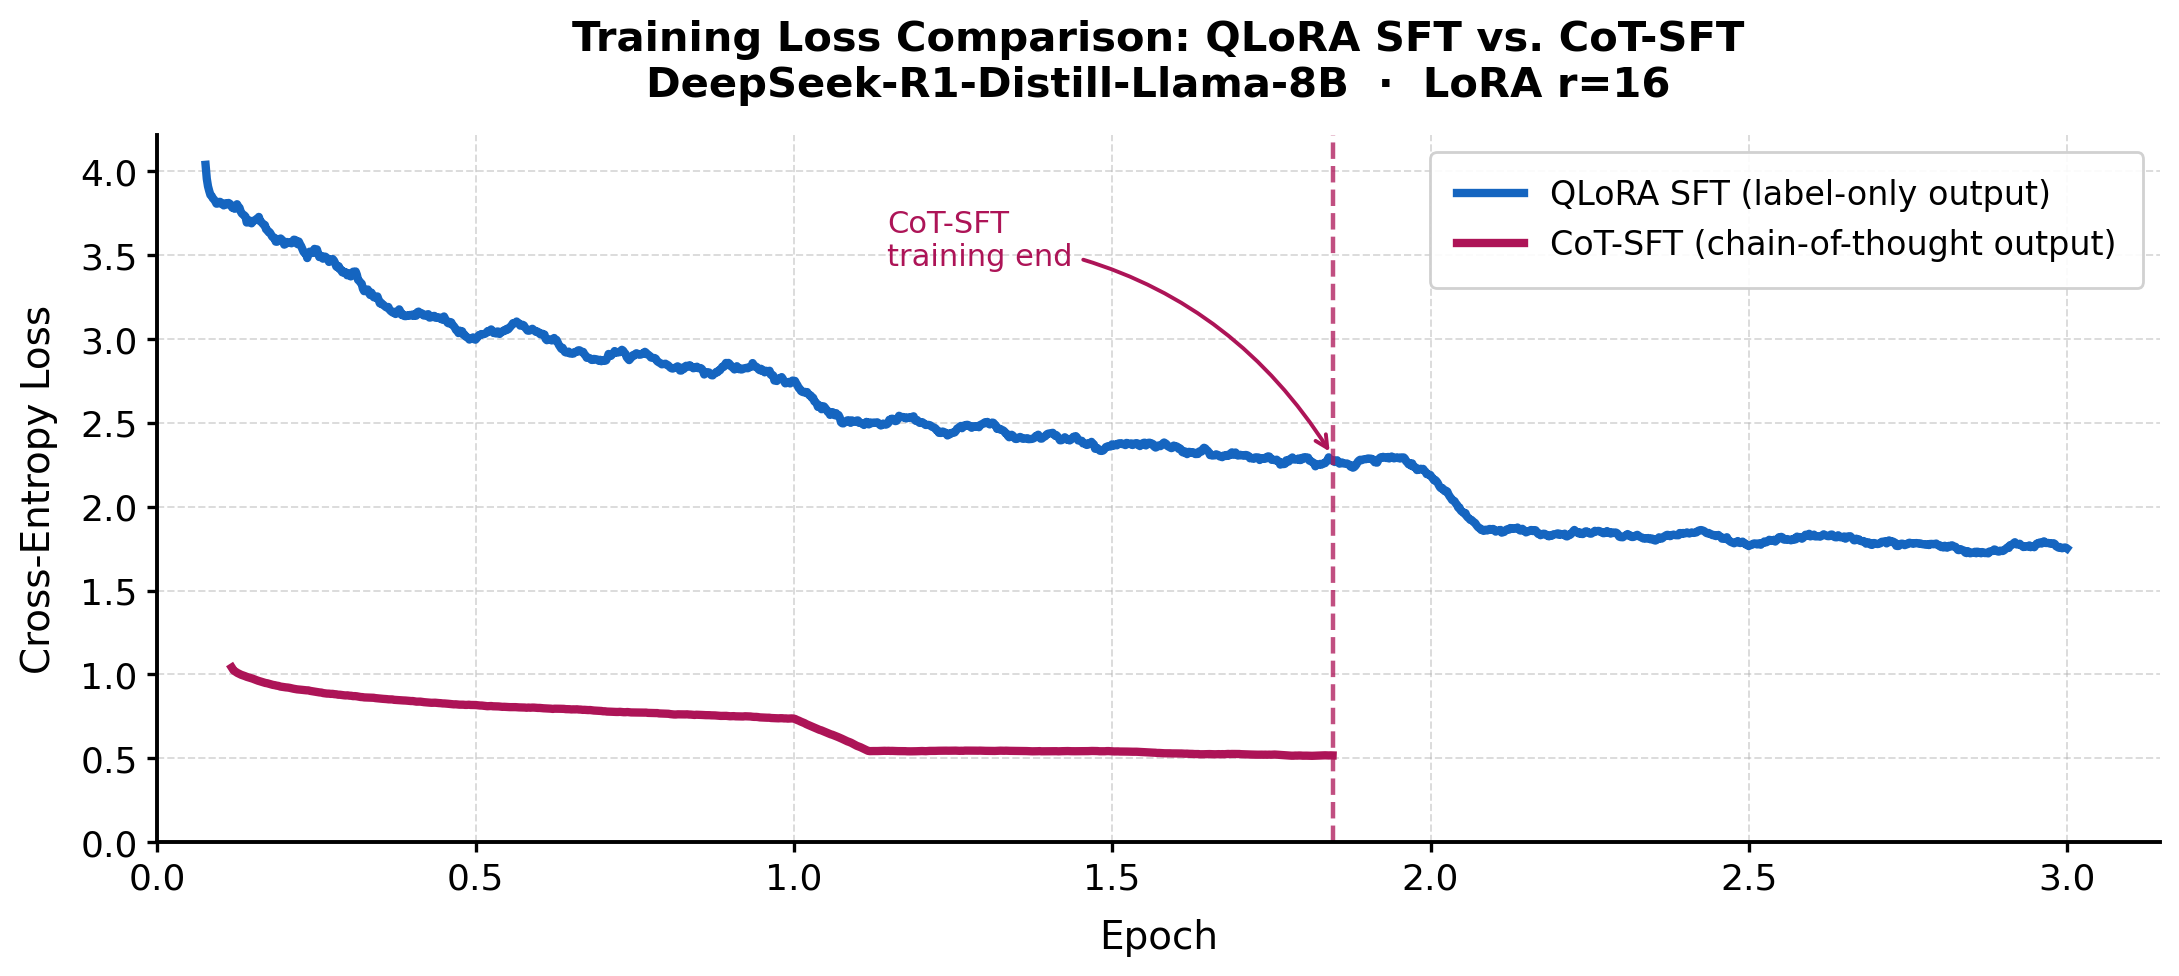
\includegraphics[width=0.82\linewidth]{../figures/fig8_qlora_vs_cotsft_loss.png}
\caption{Training loss for QLoRA-SFT (blue) and CoT-SFT (pink) on
  DeepSeek-R1-Distill-Llama-8B with LoRA $r=16$.
  The dashed line marks the end of the first stage.
  CoT-SFT converges to a lower loss owing to the richer
  chain-of-thought supervision signal.}
\label{fig:loss}
\end{figure}

% ============================================================
\section{Experiments}
\label{sec:experiments}

\subsection{Evaluation Benchmarks}

We evaluate on four benchmarks from the Open FinLLM
Leaderboard~\cite{huang2024openfinllms}:

\begin{table}[ht]
\centering
\small
\begin{tabular}{@{}llrp{5cm}@{}}
\toprule
\textbf{Benchmark} & \textbf{Domain} & \textbf{Size} & \textbf{Description} \\
\midrule
FPB   & EN News    & 393   & Financial PhraseBank; partially in-distribution \\
FiQASA & EN Q\&A   & 217   & Financial Q\&A opinions; unseen cross-domain \\
SM-BigData & Social & 1,472 & BigData22 Twitter stock movement; unseen \\
SM-CIKM    & Social & 1,143 & CIKM18 Twitter stock movement; unseen \\
\bottomrule
\end{tabular}
\caption{Evaluation benchmarks from the Open FinLLM Leaderboard.
  FPB shares its source with the training FPB split;
  the remaining three benchmarks are entirely out-of-distribution.}
\label{tab:benchmarks}
\end{table}

All models use 4-bit NF4 quantization, \texttt{max\_new\_tokens}$=32$,
and greedy decoding.
For models producing \texttt{<think>}\ldots\texttt{</think>} blocks,
the block is stripped before label extraction.

\subsection{Baselines}

Three open-source models are evaluated zero-shot:
\textbf{Mistral-7B-Instruct-v0.3} (7B),
\textbf{Meta-Llama-3-8B-Instruct} (8B), and
\textbf{DeepSeek-R1-Distill-Llama-8B} (8B) --- the backbone for FinMini.

\subsection{Main Results}

\begin{table}[ht]
\centering
\small
\setlength{\tabcolsep}{7pt}
\begin{tabular}{@{}lcccccc@{}}
\toprule
\multirow{2}{*}{\textbf{Model}} &
  \multicolumn{4}{c}{\textbf{Accuracy (\%)}} &
  \multirow{2}{*}{\textbf{Avg}} \\
\cmidrule(lr){2-5}
& \textbf{FPB} & \textbf{FiQASA} & \textbf{SM-BD} & \textbf{SM-CIKM} & \\
\midrule
Mistral-7B (zero-shot)             & 85.5 & 72.8 & 49.1 & 47.3 & 63.7 \\
Llama-3-8B (zero-shot)             & 69.5 & 82.0 & 43.1 & 39.3 & 58.5 \\
DeepSeek-8B (zero-shot)            & 83.5 & 57.6 & 55.0 & 49.3 & 61.4 \\
\midrule
FinMini QLoRA-SFT                  & 93.1 & 94.5 & 57.1 & 52.2 & 74.2 \\
\textbf{FinMini CoT-SFT (Ours)}    & \textbf{98.5} & \textbf{97.7} & \textbf{57.3} & \textbf{55.5} & \textbf{77.3} \\
\bottomrule
\end{tabular}
\caption{Accuracy on Open FinLLM Leaderboard benchmarks.
  Bold: best result per column.
  FinMini CoT-SFT outperforms all baselines on every benchmark.}
\label{tab:main}
\end{table}

Figure~\ref{fig:bar} provides a visual comparison of all five models.
FinMini CoT-SFT (pink bars, starred) achieves the highest accuracy on
all four tasks, with dramatic improvements on formal financial benchmarks
and consistent gains on social-media tasks.

\begin{figure}[ht]
\centering
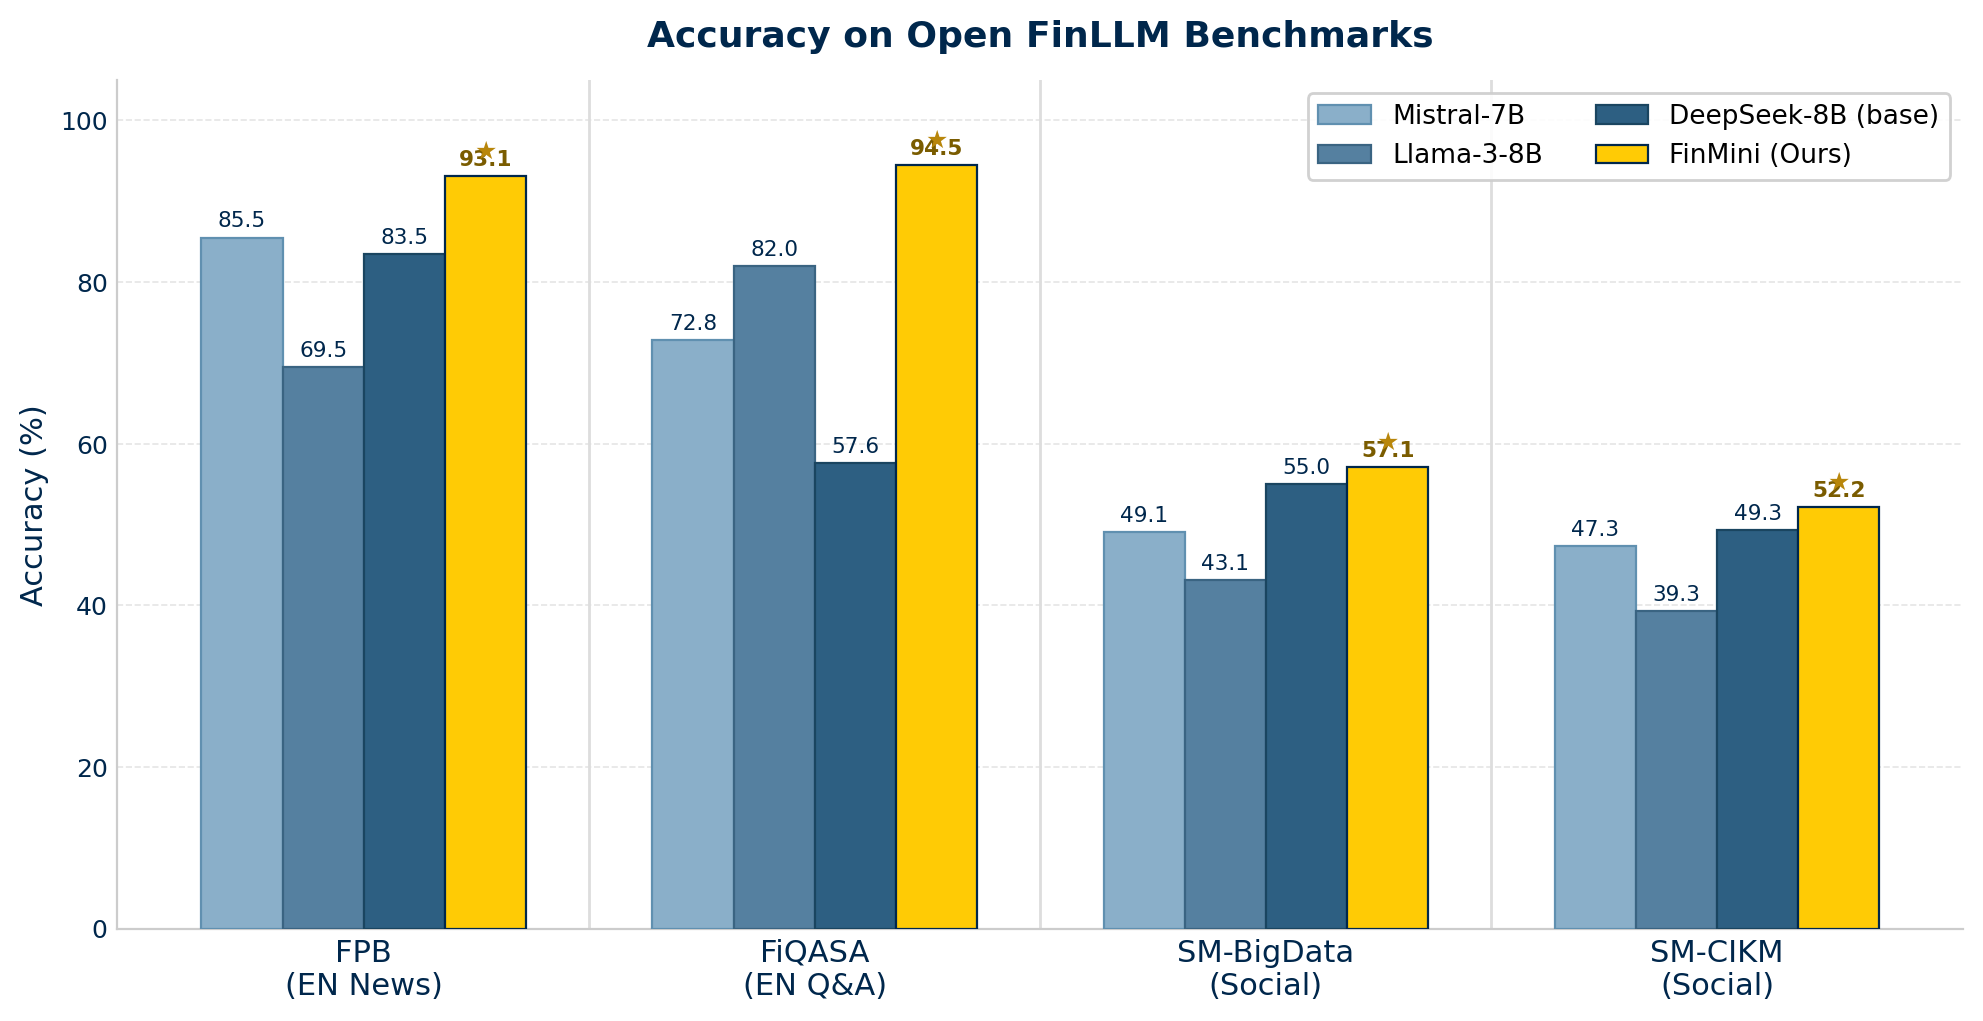
\includegraphics[width=\linewidth]{../figures/fig7_bar.png}
\caption{Accuracy on the Open FinLLM Leaderboard benchmarks.
  Stars ($\bigstar$) mark the best result per benchmark.
  FinMini CoT-SFT (pink) achieves the top score on all four tasks.}
\label{fig:bar}
\end{figure}

\subsection{Ablation: Contribution of Each Fine-Tuning Stage}

Figure~\ref{fig:ablation} visualizes the incremental accuracy gain from
each fine-tuning stage relative to the DeepSeek-8B zero-shot baseline.
Each bar is partitioned into three segments: the baseline accuracy (blue),
the gain from QLoRA-SFT (amber), and the additional gain from CoT-SFT (rose).
Dashed horizontal lines mark the baseline level for each benchmark.

\begin{figure}[ht]
\centering
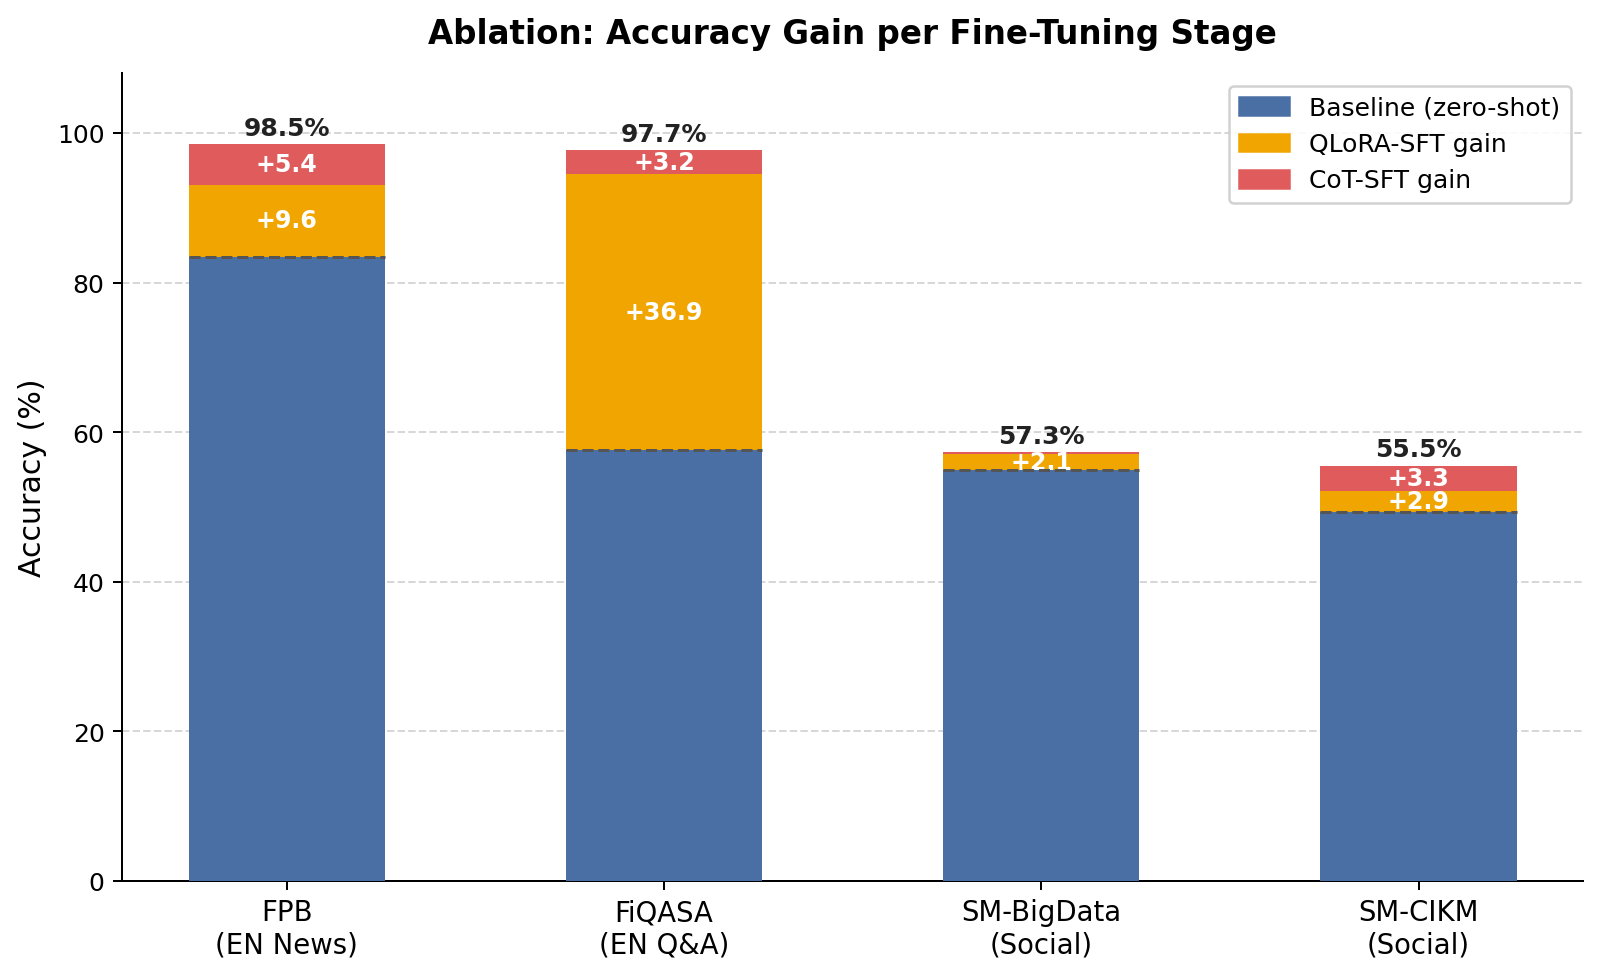
\includegraphics[width=0.92\linewidth]{../figures/fig9_ablation.png}
\caption{Stacked accuracy contributions per fine-tuning stage.
  Blue: DeepSeek-8B zero-shot baseline.
  Amber: gain from QLoRA-SFT.
  Rose: additional gain from CoT-SFT.
  Labels inside each segment show the per-stage accuracy increment (pp);
  bold labels above each bar show the final accuracy of FinMini CoT-SFT.}
\label{fig:ablation}
\end{figure}

QLoRA-SFT provides the dominant gain, particularly on FiQASA ($+36.9$ pp),
where the baseline was clearly miscalibrated for Q\&A-style financial
sentiment.
CoT-SFT adds a further $+5.4$ pp on FPB and $+3.3$ pp on SM-CIKM,
confirming that structured reasoning supervision yields consistent gains
beyond label-only training.
Social-media benchmarks improve modestly at both stages, reflecting the
limited coverage of informal financial language in the training corpus.

% ============================================================
\section{Analysis}
\label{sec:analysis}

\subsection{Why Chain-of-Thought Supervision Helps}

The gains from CoT-SFT are most pronounced on formal-language benchmarks
(FPB: $93.1 \to 98.5$\%, FiQASA: $94.5 \to 97.7$\%).
We attribute this to two complementary effects.
\textbf{Format alignment}: the base model was distilled to produce
\texttt{<think>} traces; QLoRA-SFT on label-only outputs partially
suppresses this capability, whereas CoT-SFT reinforces it.
\textbf{Reasoning quality}: structured traces force the model to
identify domain-specific sentiment cues --- hedged language in analyst
commentary, implicit expectations in earnings guidance --- before
committing to a label, reducing ambiguity-driven errors.

\subsection{The Social-Media Performance Gap}

All models exhibit a ${\sim}30$--40~pp accuracy gap between formal
financial benchmarks and social-media tasks (Table~\ref{tab:main}).
This is consistent with known challenges in social-media financial
NLP~\cite{cam2024twitter,du2024survey}: informal language, slang,
hashtags, and ticker symbols are underrepresented in instruction-tuning
corpora; sentences are shorter and more ambiguous; and class distributions
differ substantially from news-style data.
FinMini narrows the gap relative to all baselines --- SM-BigData improves
from 55.0\% (baseline) to 57.3\% (+2.3 pp), and SM-CIKM from 49.3\% to
55.5\% (+6.2 pp) --- but does not eliminate it.
Future work should incorporate Twitter and Reddit financial corpora
directly into Stage~1 training.

\subsection{LLM-Driven Long-Short Equity Strategy}

To demonstrate a practical downstream application, we deploy FinMini
CoT-SFT in a \textbf{quarterly long-short equity strategy} over the
full S\&P~500 universe.
For each stock-quarter pair, a document is assembled from the earnings
call transcript (fetched via the DefeatBeta API) and up to three recent
news articles, truncated to 3,072 tokens.
The model outputs a JSON assessment containing an \texttt{llm\_score}
(0--100), direction, confidence level, and a brief reasoning summary.

At each rebalance date (45 days after quarter-end), stocks are ranked
cross-sectionally by \texttt{llm\_score}.
The top 10\% are held long and the bottom 10\% are held short, both
equal-weighted, over a 12-quarter backtest window.
This application illustrates that domain-adapted LLM sentiment signals
can extract forward-looking information from unstructured financial
documents at scale, extending the model's utility beyond classification
accuracy to a real-world portfolio construction task.

% ============================================================
\section{Conclusion}
\label{sec:conclusion}

We presented FinMini, a two-stage domain adaptation pipeline that
transforms a compact 8B reasoning-distilled LLM into a
state-of-the-art financial NLP model.
QLoRA-SFT establishes strong domain-specific accuracy on formal
financial benchmarks, and CoT-SFT pushes performance to near-ceiling
levels (98.5\% on FPB, 97.7\% on FiQASA) by reinforcing structured
reasoning aligned with the model's native output format.
FinMini outperforms all tested general-purpose baselines across all four
Open FinLLM Leaderboard benchmarks.

Three key takeaways emerge from this work.
First, reasoning-distilled models provide a better initialization for
financial NLP than standard instruction-tuned models of similar scale,
even before fine-tuning.
Second, CoT supervision significantly outperforms label-only SFT on
formal financial text; both stages are necessary for peak performance.
Third, social-media financial tasks remain the hardest category for
all models, requiring dedicated training data and future work on
informal-language robustness.

% ============================================================
\section*{Author Contributions}

\textbf{JiaYuan Jiang} optimized the training codebase for performance
and reliability, including implementing an automatic checkpoint and
resume mechanism to handle interruptions on shared GPU clusters.
Deployed the full training pipeline on the University of Michigan
Great Lakes HPC cluster.
Tuned training hyperparameters (learning rate, batch size, LoRA rank,
gradient accumulation) to improve convergence.
Analyzed training dynamics and evaluation results across all benchmarks.
Designed and produced the conference poster.
Authored the final project report.

\textbf{JiaYi Zhang}: \textit{(details to be filled in)}

\textbf{Yue Yu}: \textit{(details to be filled in)}

\textbf{YiXiang Fei}: \textit{(details to be filled in)}

% ============================================================
\bibliographystyle{plain}
\bibliography{../poster/poster_new}

\end{document}
